\documentclass[12pt]{article}
\usepackage[utf8]{inputenc}
\usepackage[T1]{fontenc}
\usepackage{amsmath,amsfonts,amssymb}
\usepackage{graphicx}
\usepackage{a4wide}
\usepackage{hyperref}
%\usepackage[style=numeric-comp]{biblatex}
\usepackage{enumerate}

\newcommand{\D}{{2^Q}}
\newcommand{\bw}{\mathbf{w}}
\newcommand{\bwT}{\mathbf{w}^\mathsf{T}}
\newcommand{\T}{^\mathsf{T}}
\newcommand{\bphi}{\boldsymbol{\varphi}}
\newcommand{\bx}{\mathbf{x}}
\newcommand{\bc}{\mathbf{c}}
\newcommand{\bd}{\mathbf{d}}

\begin{document}
\begin{center}
{\Huge\bf Aloha collision detector}
\end{center}

%\title{}
% The author is grateful to the readers for consistent problem statement.}}
%\author{Vadim Strizhov}%\footnote{E-mail: vadim.vct@gmail.com}}
%\date{}
%\maketitle

\begin{quote}
This one-page report\footnote{By Vadim Strijov,\href{mailto:vadim.vct@gmail.com}{\texttt{vadim.vct@gmail.com}}, 7/2/2025} describes a collision detection classifier model. It delivers satisfactory accuracy of collision detection, the expectation of $\text{AUC} = 0.97$. It is simple and portable to an RFID reader. {\bf \emph{\hyperref[sec:experiment]{The link to code}}} is in Appendix.
\end{quote}

%\noindent \textbf{Keywords:} machine learning; aloha collision; collision detection; radial basis function; self-modeling regression; additive regularization

\paragraph{Probability of a collision in a slot.} The probability zero, one, two, and three or more transmitters sharing a given slot for~$N$ transmitters and $2^Q$ allocated time slots is 
%\newcommand{\D}{{2^Q}}
\[
P_0 = \left( \frac{\D-1}{\D} \right)^N, 
P_1 = N \times \frac{1}{\D} \times \left(\frac{\D-1}{\D}\right)^{N-1},
P_2 = \frac{N(N-1)}{2}  \times \frac{1}{2^{2Q}} \times \left(\frac{\D-1}{\D}\right)^{N-2},
\]
and $P_{\geq 3} = 1 - P_0 - P_1 - P2$. 

\paragraph{The classifier model description.} The proposed collision detection classifier model is the superposition of logistic regression, radial basis functions with Gaussian kernels, and self-modeling regression. %For the simplicity of the computations %and signal processing procedures, most part of 
The model acts in the complex space.

\paragraph{The dataset creation.} Four classes were created: no-signal class with noise, a single transmission, exactly two collided transmitters, and from thee to five collided transmitters. The data sample size and the signal mixture scaling keep characteristics of the orginal data. To simulate signal attenuation, weighted coefficients were used.

\paragraph{The classifier accuracy analysis.} The logistic regression returns the probability of collision, so the Area Under ROC is its quality criterion. Its expected value is 9.7. It means a reasonable probability of Aloha collision detection for one versus two transmitters. 

\paragraph{Maximizing the accuracy on prior knowledge of $N,Q$.} %It is suggested to use predefined optimal parameters~$\bw_\text{opt}$, suitable for the current session or environment and use Bayesian apporoach to use prior knowlede in the optimization criterion:
%\[
%\mathcal{L}= \sum_{i=1}^m \biggl( y_i \log p(\bx_i,\bw) + (1-y_i) \log\bigl(1-p(\bx_i, \bw)\bigr)\biggr)+ \frac{1}{2}(\bw-\bw_\text{opt})\T\mathbf{A}^{-1}(\bw-\bw_\text{opt}).
%\]
The collision classifier model was tested on datasets with various sample sizes and class balance ratios. The test shows that the accuracy is stable around borderline values of the sample size and class balance ratio. The AUC varies in~$0.90,\ldots,0.97$ (for balanced~$0.94,\ldots,0.98$) on the test data. 

\paragraph{Model portability analysis.} The preliminary number of  operations: projection \texttt{complex}: $K \times T \times 2S$ multiplications, distance  \texttt{complex}: $K \times T$  multiplications. The required memory \texttt{complex}: $128\times 39$.  For~$K=128$, $T=39$, and  $S=1$ the model could be ported to the RFID reader after feasible simplificaton.

\paragraph{Future considerations.} The problem of signal separation of two transmitters is important. Accorting to the obtained results it seems to be feasible even for a single reader.
 
\paragraph{Reproducibility of the experiment. } The Google Colab Python notebook is accessible by  {\bf \emph{\hyperref[sec:experiment]{the link in  Appendix}}} with detailed instructions how to run the experiment.

\clearpage 

\begin{center}
{\Huge\bf Appendix}
\end{center}
\section{Probability of a collision in a slot}
There allocated~$2^Q$ time slots for the set of~$N$ RFID tags, or transmitters. For a single transmitter the probability to occupy the empty slot is~$\left( \frac{1}{D} \right)$. For simplicity denote~$Q = \log_2 D$.

% There is a group of N people with their birthdays.
% Determine the probability of the day with no birthdays. 
% Determine the probability of the day having exactly two birthdays.
% Determine the probability of the day having exactly three or more birthdays.
% Let's analyze the probability of birthday occurrences for a group of  N  people, assuming that birthdays are uniformly distributed across 365 days (ignoring leap years).

\paragraph{Probability of a slot having no transmitters.}  Each transmitter's time slot is independently and randomly chosen from~$D$ slots. The probability that a specific slot is not occupied by a \emph{specific} transmitter is $\frac{D-1}{D}$. Since there are~$N$ transmitters, the probability that a specific slot is not occupied by anyone is
\[
P_0 = \left( \frac{D-1}{D} \right)^N.
\]
\paragraph{Probability of a slot having exactly two transmitters.}
To determine the probability that exactly two transmitters occupy a given slot, estimate the probability that a specific transmitter occupies this slot, $\frac{1}{D}$. The probability that exactly two specific transmitters occupy that slot is 
$\left(\frac{1}{D}\right)^2$, while the remaining~$N-2$ transmitters \emph{do not} occupy that slot, which occurs with probability $ \left(\frac{D-1}{D}\right)^{N-2} $.  Since any two of the \( N \) transmitters can be the ones sharing the slot, we choose two transmitters from~$N$, which gives %the binomial coefficient~
$\binom{N}{2} = \frac{N(N-1)}{2}$.
Thus, the probability of exactly two transmissions in a given slot is:
\[
P_2 = \binom{N}{2} \left(\frac{1}{D}\right)^2 \left(\frac{D-1}{D}\right)^{N-2}
= \frac{N(N-1)}{2}  \times \frac{1}{D^2} \times \left(\frac{D-1}{D}\right)^{N-2}
\]
\paragraph{Probability of a slot having three or more transmitters.} The probability of exactly three transmitters occupying a given slot (while the others don't) is
\[
P_3 = \binom{N}{3} \left(\frac{1}{D}\right)^3 \left(\frac{D-1}{D}\right)^{N-3}
= \frac{N(N-1)(N-2)}{6} \times \frac{1}{D^3} \times \left(\frac{D-1}{D}\right)^{N-3}.
\]
The probability of four, five, or more transmitters occupying the same slot follows similarly. Thus, the probability of three or more transmitters sharing a given slot is
$ %\[
P_{\geq 3} = 1 - P_0 - P_1 -P_2,
$ %\]
where the probability of exactly one transmitter occurring is
\[
P_1 = N \times \frac{1}{D} \times \left(\frac{D-1}{D}\right)^{N-1}
\]

\begin{figure}[!tb]
\centering
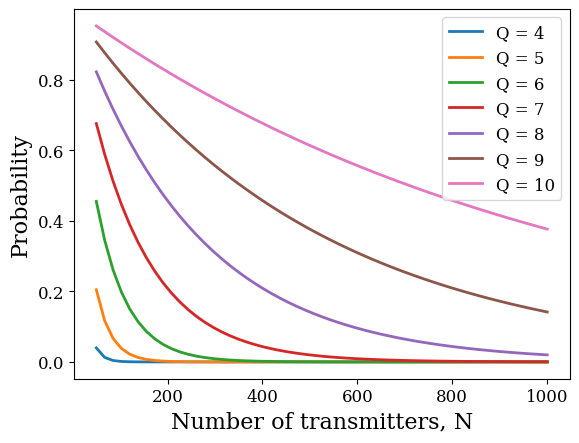
\includegraphics[width=0.45\textwidth]{fig_P0}
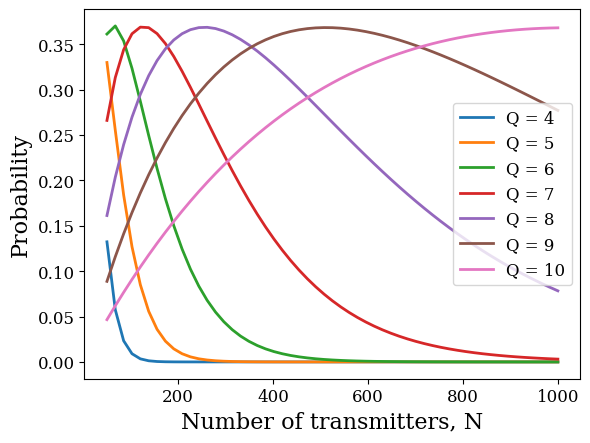
\includegraphics[width=0.45\textwidth]{fig_P1}\\
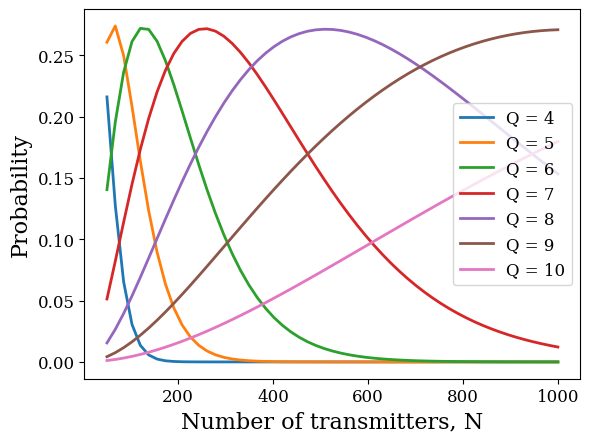
\includegraphics[width=0.45\textwidth]{fig_P2}
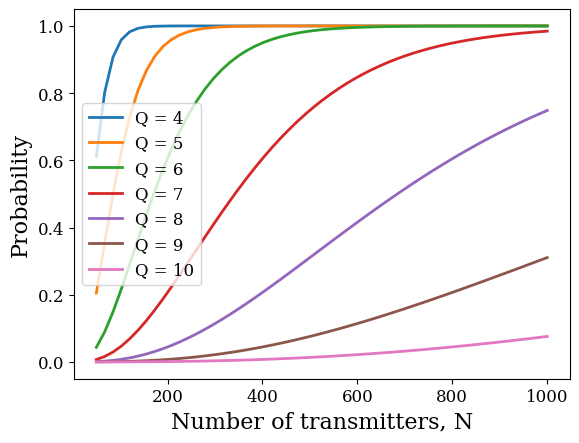
\includegraphics[width=0.45\textwidth]{fig_P3}\\
\caption{Probalility of no transmitter occupies a slot depends on the number of transmitters~$N$ and the number of slots~$D$. The top left is~$P_0$ (no transmission in a slot), right is~$P_1$ (one transmission), the bottom left is~$P_2$ (two transmitters collide), and right is~$P_3$ (three and more transmitters collide).}
\label{fig:pr_p0}
\end{figure}

And since no transmission, exactly one transmission, or at least two transmission must occur on any given slot, we get:
\[
P_{\geq 3} = 1 - P_0 - P_1 - P_2 
\]
This formula provides the probability of at least three transmitters sharing a specific slot.

The plots in Figure~\ref{fig:pr_p0} show the fact that is if 
with an insufficiently small number of slots, there is no initial period where the probability of getting two transmitters in one slot increases. That is, if there are enough transmitters to overlap at all, they will \emph{immediately start crowding into multiple transmissions per slot.} This fact brings importance to detect~${\geq 3}$  collisions. We follow up this consideration in Section~\ref{ICA}.

In terms of the variables~$N$ and $Q$ the answer will be 
\[
P_0 = \left( \frac{\D-1}{\D} \right)^N, 
P_1 = N \times \frac{1}{\D} \times \left(\frac{\D-1}{\D}\right)^{N-1},
P_2 = \frac{N(N-1)}{2}  \times \frac{1}{2^{2Q}} \times \left(\frac{\D-1}{\D}\right)^{N-2},
\]
and $P_{\geq 3}$  as above. This collision problem is known as the probabilistic birthday paradox~\cite{Sun2021,Santos2015,Mosteller1962,Shakiba2014}.


\section{The classifier model description}

\begin{figure}[!bp]
\centering
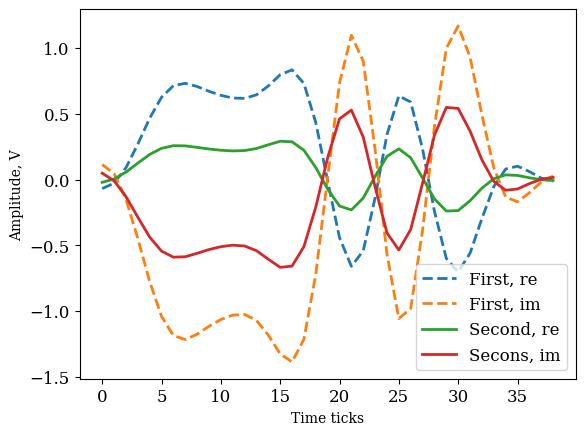
\includegraphics[width=0.45\textwidth]{fig_amplitude_scaled_distance}
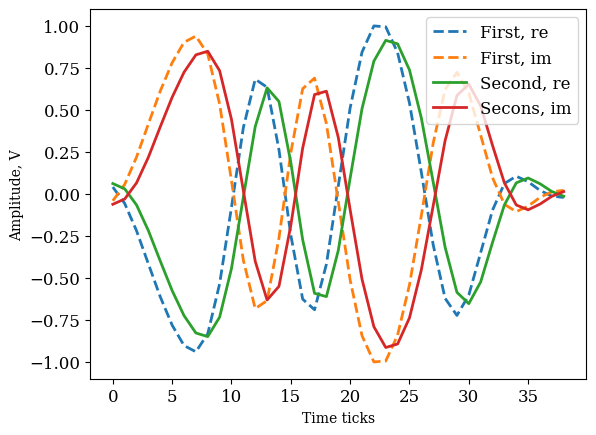
\includegraphics[width=0.45\textwidth]{fig_centroid_still_in_cluster}
\caption{The self-modeling regression regresses a signal to centroid as a projection (left), while shifting the phase of the whole I/Q data signal to find the best fit (right). The legend shows real (re) and imaginary (im) part of the complex signal. The dashed line (First) shows the centroid, the solid line (Second) sows the approximated signal.}
\label{fig:projected_shift}
\end{figure}

The proposed collision detection classifier model is the superposition of logistic regression, radial basis functions with Gaussian kernels, and self-modeling regression. The first part returns the probability of collision as
\[
p(y|\bw) =\bigl( 1+\exp(-\bwT\bphi(\bx)) \bigr)^{-1}.
\]
The second part is the vector function~$\bphi(\bx)$ with Gaussian kernels 
\[
\bphi = [\varphi_1,\ldots,\varphi_K]\T, \quad \text{where} \quad \varphi_k(\bx) =  \exp\left(-\frac{\|\bd(\bx, \bc_k) - \bc_k\|^2}{2\sigma_k^2}\right).
\]
And the last part is the self-modeling regression. It approximates the signal~$\bx$ with the centroid~$\bc$ as
\[
\hat{\bc} = v_1 \bigl( \text{phase shift}(\bx, v_2)\bigr),
\]  
with two parameters~$v_1,v_2$. The first parameter~$v_1$ is calculated as the dot product ratio of the projection 
\[
\text{proj}_\bc \bx = \frac{\bc\T\bx}{\bc\T\bc}\bc, \quad \text{as long as} \quad \bx \neq \boldsymbol{0}.
\]
Note that this ratio could be negative, which is an admissible operation for the I/Q data signal. The second parameter calculated as an argument of minimum distance
\[v_2 =\mathop{\arg\min}\limits_{\text{admissible shift}}\|\hat{\bc}-\bc\|^2.\]

For the simplicity of the computations and signal processing procedures, most part of the model acts in the complex space. The variables $\bx, \bd, \bc \in \mathbb{C}^T$,
where~$T$ is the length of the transmitted I/Q data signal, 
$\bphi, \bw \in \mathbb{R}^K$,
where~$K$ is the number of centroids, and the class~$y\in\{0,1\}.$ The in-phase part of the complex vector~$\bx$ is real, while the quadrature part is imaginary.

Figure~\ref{fig:projected_shift} illustrates the self-modeling regression. The first, dashed, signal is the centroid, scaled to 1\,V, and the second, solid, signal is modified to approximate the centroid.

\section{The dataset creation}
The signal mixture procedure is organized as follows. The initial data seems to be scaled already and the scale does not always follow the amplitude in the $0.3,\ldots,1.1$\,V segment. However, the signal at the given scaling seems decent. The same with the noise. Its level is assumed to be properly set, so we leave it unchanged. The signal of small energy will express a bigger influence of the noise at the reader, so unchanging the given settings seems to be a natural decision. 
 
Adding the signal increases their power for the same-phase case. To make the problem a little bit harder (signal attenuates with distance) we set the summing coefficients less than one: $0.5,\ldots,0.8$ fixing them for the experiment. The scaling $A_\text{result} = \left| \sum_{i=1}^{N} A_i \exp({j\phi_i}) \right|$, where $A$ are the amplitudes of the signals and $\phi$ is the phase difference between them~\cite{Balanis2005} (we find this with Gilbert transform, if the model complexity allows)  requires additional discussion.

The generated data sample size. Decoupling indexes of data and noise datasets and assuming that the mixture of Gaussian noise is the Gaussian noise with zero expectation could provide us with a big sample size. We set the size of the original data for each of the four classes.  In the case of~$\geq 3$ classes the mixture of 3 to five signals was generated.

\section{The classifier accuracy analysis}

Since the logistic regression model returns the probability of collision, the Area Under ROC is assigned as the quality criterion. For various cross-validations, its expected value is 9.7. For various normally-balanced datasets, it varies in the segment~$0.94,\ldots,0.98$. It means a reasonable probability of Aloha collision detection for one versus two or more transmitters. 

\begin{figure}[!tb]
\centering
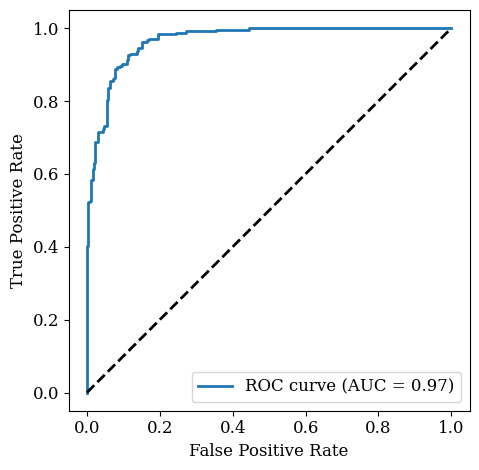
\includegraphics[width=0.4\textwidth]{fig_ROC_1v2}
\caption{The model returns the probability of collision detection. The higher Operator Reciever Curve shows the better quality of detection (one transmitter versus two) on the \emph{test part} of the dataset.}
\label{fig:AUC_1v2}
\end{figure}

Figure~\ref{fig:AUC_1v2} shows the accuracy for the classification single transmitter versus the collision of two transmitters. The overall classification procedure is organized in the following way. The one-versus-all four classes classification problem is listed according to their probability: empty versus any transmission, one versus two transmitters, one versus two or more transmitters. The detection of three or more against two or more requires the blind signal separation procedure, which is introduced in Section~\ref{ICA}.

\section{Maximizing the accuracy on prior knowledge of $N,Q$}

Assume as the prior knowledge 1)~that the sufficient number of allocated for transmission time slots~$2^Q$ brings a small number of collisions of two and a lesser number of collisions of 3+ transmitters and, 2)~the model parameters are subject to optimization during the reader's session. In this case, we suggest using predefined optimal parameters~$\bw_\text{opt}$, suitable for the current session or environment. For the model parameter optimization, apply a Bayesian penalty function for the current model. According to the Bayes' rule
\[
p(\bw|y,\bx) \propto p(y|\bw,\bx) p({\bw}_\text{opt}),
\]
it changes the most likely parameters~$p(y|\bw,\bx)$ for the most probable parameters~$p(\bw|y,\bx$. So the optimization criterion is 
\[
\mathcal{L}= \sum_{i=1}^m \biggl( y_i \log p(\bx_i,\bw) + (1-y_i) \log\bigl(1-p(\bx_i, \bw)\bigr)\biggr)+ \frac{1}{2}(\bw-\bw_\text{opt})\T\mathbf{A}^{-1}(\bw-\bw_\text{opt}).
\]
The covariance matrix~$A$ is estimated in the multiple cross-validation procedure using prior knowledge datasets. The \texttt{LogisticRegression} model from \texttt{sklearn} has the regularization component (the right part of this formula)  with~$\bw_\text{opt}=\boldsymbol{0}$ and $\mathbf{A} = \alpha\mathbf{I}$ by befault. 

Test the suggested collision classifier model on datasets with various sample sizes and class balance ratios. 
The approximate parameters for~$N$ and~$Q$ simulation were taken from the paper~\cite{Kang2011}. So let the number of single transmissions varies from 100 to 1000, and the ratio of collided transmission varies from 0.1 to 0.9.

\begin{figure}[!htbp]
\centering
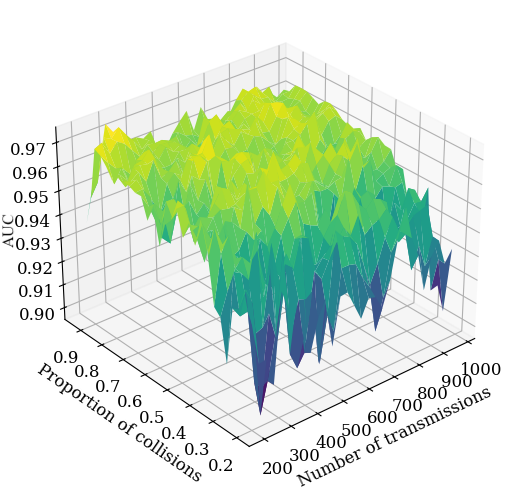
\includegraphics[width=0.6\textwidth]{fig_sampe_size_mean2}
\caption{The accuracy of collision detection depends on the dataset sample size and class imbalance.}
\label{fig:samle_size}
\end{figure}

Figure~\ref{fig:samle_size} illustrates \emph{the class balancing} problem. It shows that the accuracy is stable around borderline values of the sample size and class balance ratio. It varies in the segment~$0.90,\ldots,0.97$ for training data. Each point of the surface is an independent train-test cycle for the regression model. The right axis shows the sample size for the single-transmission class. The left axis shows the proportion of this value in the collision class. So the summary of these two values makes the size of the dataset. 

Since to optimize the model parameters we use the Newton-Raphson algorithm~\cite{Motrenko2014} that has small computational complexity and has good convergence to the optimal parameters, it could be ported to the reader. In this case, we suggest using the optimization criterion~$L$ to improve the imbalance of classes.  

However, this suggested model has equal centroids according to the assumption that different transmitters has equal probability to act on the reader's request. So we suggest to fix the parameters of the model to their equal values. In this case, there is no need to optimize the model parameters in the reader. 

\section{Model portability analysis}
To classify one transmitted signal the model uses the following operations:
\begin{enumerate}[1)]
\item projection \texttt{complex}: $K \times T \times 2S$ multiplications,
\item shifting \texttt{complex}: $K \times T \times 2S$ additions,
\item distance  \texttt{complex}: $K \times T$ additions and multiplications,
\item classification \texttt{float}: $T$  multiplications,
\item not counting single operations and padding,
\item there is \texttt{float}: $K+1$ exponent operations.
\end{enumerate}
Assuming the number of centroids~$K=128$, the length of the I/Q data signal $T=39$, and the admissible phase shift parameter is~$\pm$ time ticks, $S=10$. % 2*K*T*S+K*T. 
With a single projection procedure~$S=1$, it takes $128\times 39 \times 2$ operations. In this case the expected AUC=9.3. However, without significant loss of accuracy, we could downsample I/Q data to the required number of operations. Providing the Gaussian noise expectation is zero, no denoising and additional operations are required. Also, since the logistic regression model parameters are assumed to be equal, we can classify the values of the kernel function by threshold. 
The model requires memory \texttt{complex}: $128\times 39$. % Memory for for 3+ classes takes~$128^2*39.$ 
These estimations are preliminary. 

\section{Future considerations}\label{ICA}
For the majority of models, the pair of two transmitters versus 3+ transmitters will not give accuracy that could be used in practical applications. However, models that could perform a blind signal separation could be useful not only to detect this type of collision but also to decode the signal at the receiver for two transmitters. Since the mixture of two or more signals from a single reader is inseparable, the challenge is to find a way to separate two signals with an accuracy high enough to tell that in case of sprotting error the model declares the signal from 3+ transmitters.

We use the methods of Independent Component Analysis and Blind Signal Separation in the time domain and frequency domain~\cite{Hyvaerinen2000,Elliott1999} of the I/Q data signal using a single reader (though this method requires at least two readers, and we do not count one reader has four antennas). 

\begin{figure}[!b]
\centering
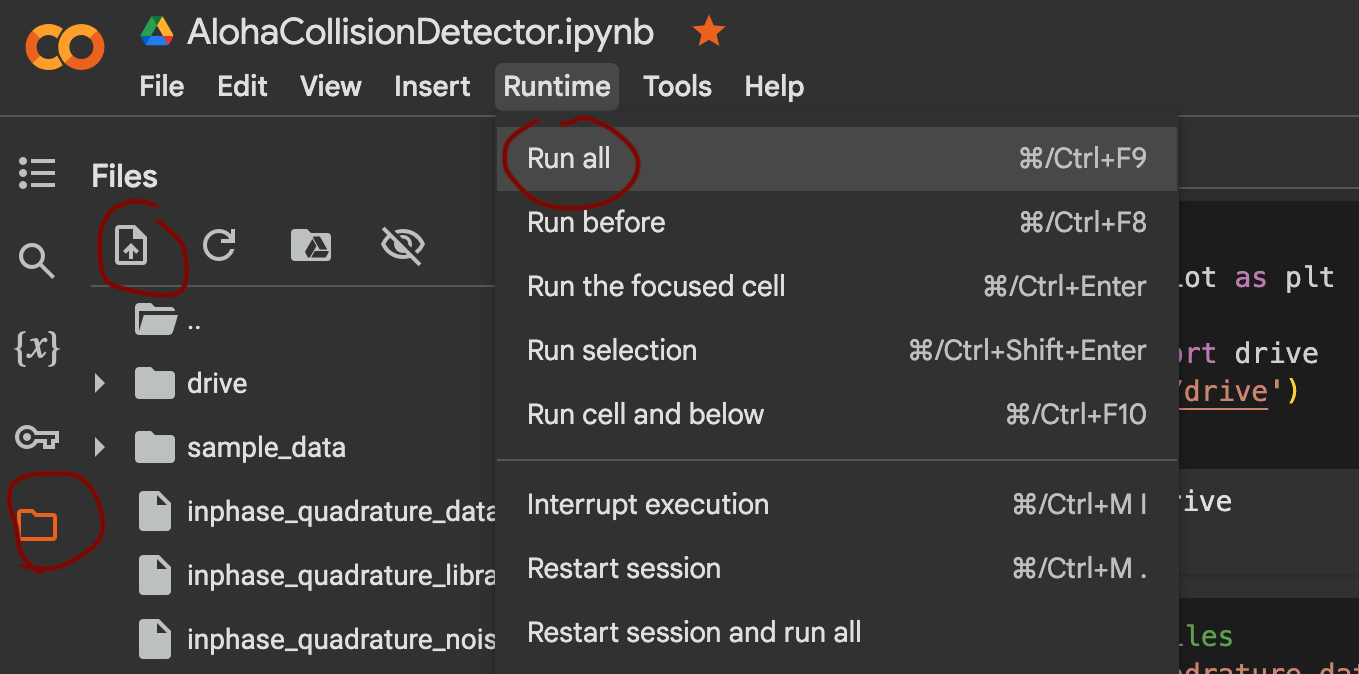
\includegraphics[width=0.5\textwidth]{fig_demo_upload}
\caption{Upload the files to Google Colab Python notebook and run the computational experiment.}
\label{fig:demo}
\end{figure}

\section{How to run the experiment}\label{sec:experiment}
\href{https://colab.research.google.com/drive/1wWEw8jcj8logartpd89VT_bX1jcP_VBb?usp=sharing}{Open the link to the Google Colab file} or copy the address to the browser:
{\footnotesize
\begin{verbatim}https://colab.research.google.com/drive/1wWEw8jcj8logartpd89VT_bX1jcP_VBb?usp=sharing\end{verbatim}}
\noindent
Press the ``Files'' icon on the left panel of Colab (the fifth from the top, below the key). Then press the ``Upload to session storage'' icon right below the word ``Files''.  From your local disk upload the files \textsf{inphase\_quadrature\_data.json}, \textsf{inphase\_quadrature\_noise.json}, and \textsf{inphase\_quadrature\_lib.npy}. The last one is attached along with this text. In the Colab menu click ``Runtime'' and select the item ``Run all''. After the first cell runs, Colab asks the access to the uploaded files. Press the button ``Continue'' each time to let the Google Colab access your Google Disk, \emph{there will be several consequent requests}. The experiment runs until the end. Figure~\ref{fig:demo} shows the orange ``Files'' icon and the ``Runtime'' menu open.\sloppy{}
%The link is %\textsf{https://colab.research.google.com/drive/1wWEw8jcj8logartpd89VT_bX1jcP_VBb?usp=sharing}

\bibliographystyle{unsrt}
\bibliography{CollisionDetector}
\end{document}





